\chapter{Related Work}
\label{cha:RelatedWork}

Public transportation navigation apps help commuters plan, track and complete their journeys more efficiently. 
While many apps provide route tracking, the challenge of knowing exactly when to get off at the right stop persists for passengers.
Without clear alerts, passengers must constantly monitor their route which can be inconvenient or impractical, especially in unfamiliar areas.
This chapter examines three popular transit apps and their approaches to notifying users when to exit.

\section{Google Maps}
Google Maps, developed by Google, is a mapping service that offers route planning across different transportation modes including driving, walking, cycling and public transit. 
The platform partners with numerous public transportation providers worldwide to integrate their data while also collecting independent information to facilitate trip planning for users.
Google Maps provides real-time transportation information that allows users to view live arrivals for buses, metros and subway systems and alerts them to canceled routes.

In 2017, Google introduced a feature for Android that sent users notifications when to transfer or exit their bus or train.
Shortly after, various online sources reported the feature's availability, and in the 2017 version of the Google Maps app, it could be enabled after selecting a public transit route.
As noted by The Verge \cite{verge_google_maps_2017}, users could toggle on reminders for departure and transfers under the "Add a Google Maps reminder" section.
However, in the 2025 version of the app, only the "Remind you to leave on time" toggle remains, with no trace of the stop alert feature in the settings.
This suggests that Google Maps has discontinued the feature.

According to 9to5Google \cite{google_maps_live_activity}, Google Maps began testing the Live Activities feature on iPhones in 2023, enabling users to receive navigation updates directly on their lock screens and in the Dynamic Island.
While helpful for navigation, this feature does not include explicit alerts for when to get off a bus or train.
Additionally, Live Activities is not yet available globally and its rollout has been limited.
Some users have reported seeing it appear intermittently, but Google has not provided an official method to manually enable it.
When activated automatically, it appears as shown in Figure~\ref{fig:GoogleMaps} (right).

\begin{figure}[htbp]
    \centering
    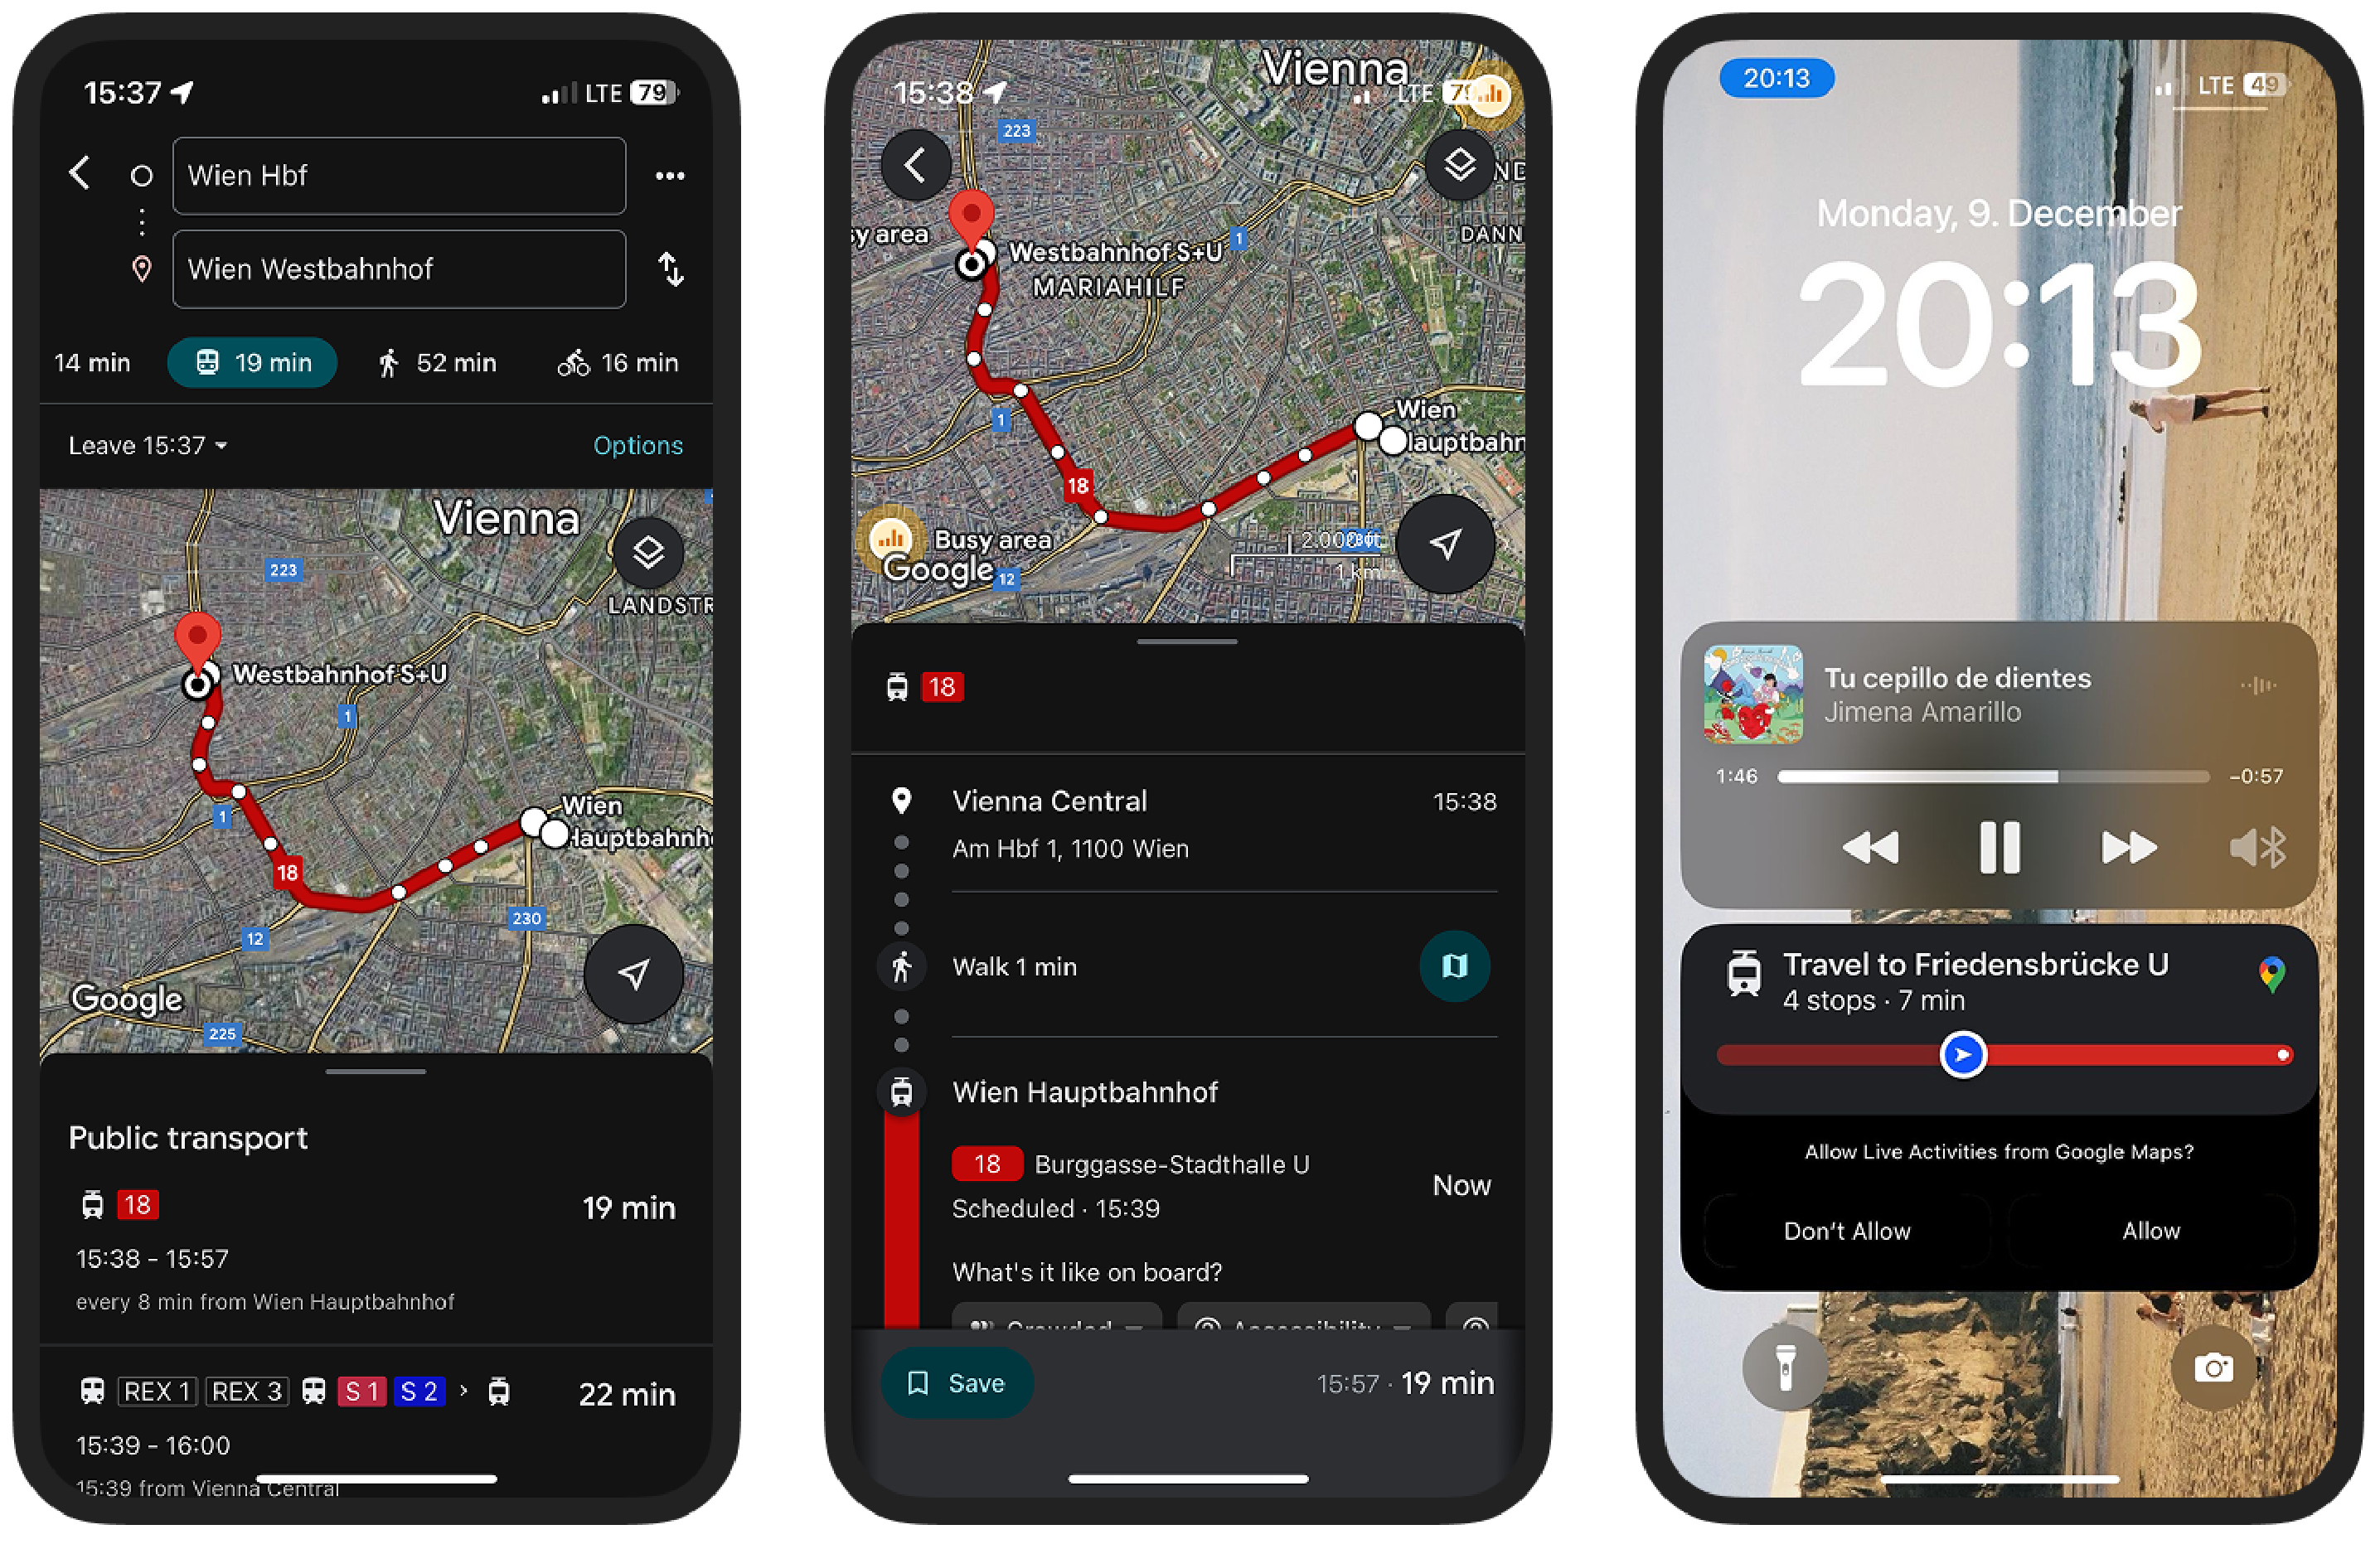
\includegraphics[width=0.35\textwidth]{GoogleMaps.pdf}
    \caption{Google Maps' Live Activities feature on iOS}
    \label{fig:GoogleMaps}
\end{figure}

\section{Citymapper}
Citymapper was founded in 2011 by former Google employee Azmat Yusuf, who aimed to simplify navigation for London's public transport system, as highlighted by TechRound \cite{citymapper_profile}.
Initially launched as Busmapper, the app focused on London's bus network but later expanded to include the underground, trams and other transport modes, eventually becoming Citymapper.
As of 2025, the platform has over 50 million users worldwide and operates in over 100 cities worldwide including New York, Paris, Tokyo, Vienna and Sydney, according to their website \cite{citymapper_cities}.
Additionally, it supports entire regions like Scotland, the Basque Country and the Balearic Islands.

The app suggests the fastest, most convenient public transport routes while considering delays and disruptions and offers users the possibility to receive notifications for service alerts.
After selecting a public transportation route, users can activate the Live Activities feature and receive notifications reminding them when to get off a bus or train.
Citymapper refers to these notifications as "Get Off Alerts", as stated on their website \cite{citymapper_getoffalerts}, and users receive three notifications at different points along their journey for better awareness.
However, testing revealed that Citymapper frequently lost location signal even in open-sky conditions, leading to missed notifications.
Additionally, while Get Off Alerts notify users when to exit, Citymapper does not provide an actual alarm, meaning users must rely solely on notifications that could be missed if the device is on silent mode or if location tracking fails.
Citymapper's Live Activities feature is displayed in Figure~\ref{fig:Citymapper} (left) and a stop notification is shown in Figure~\ref{fig:Citymapper} (right).

\begin{figure}[htbp]
    \centering
    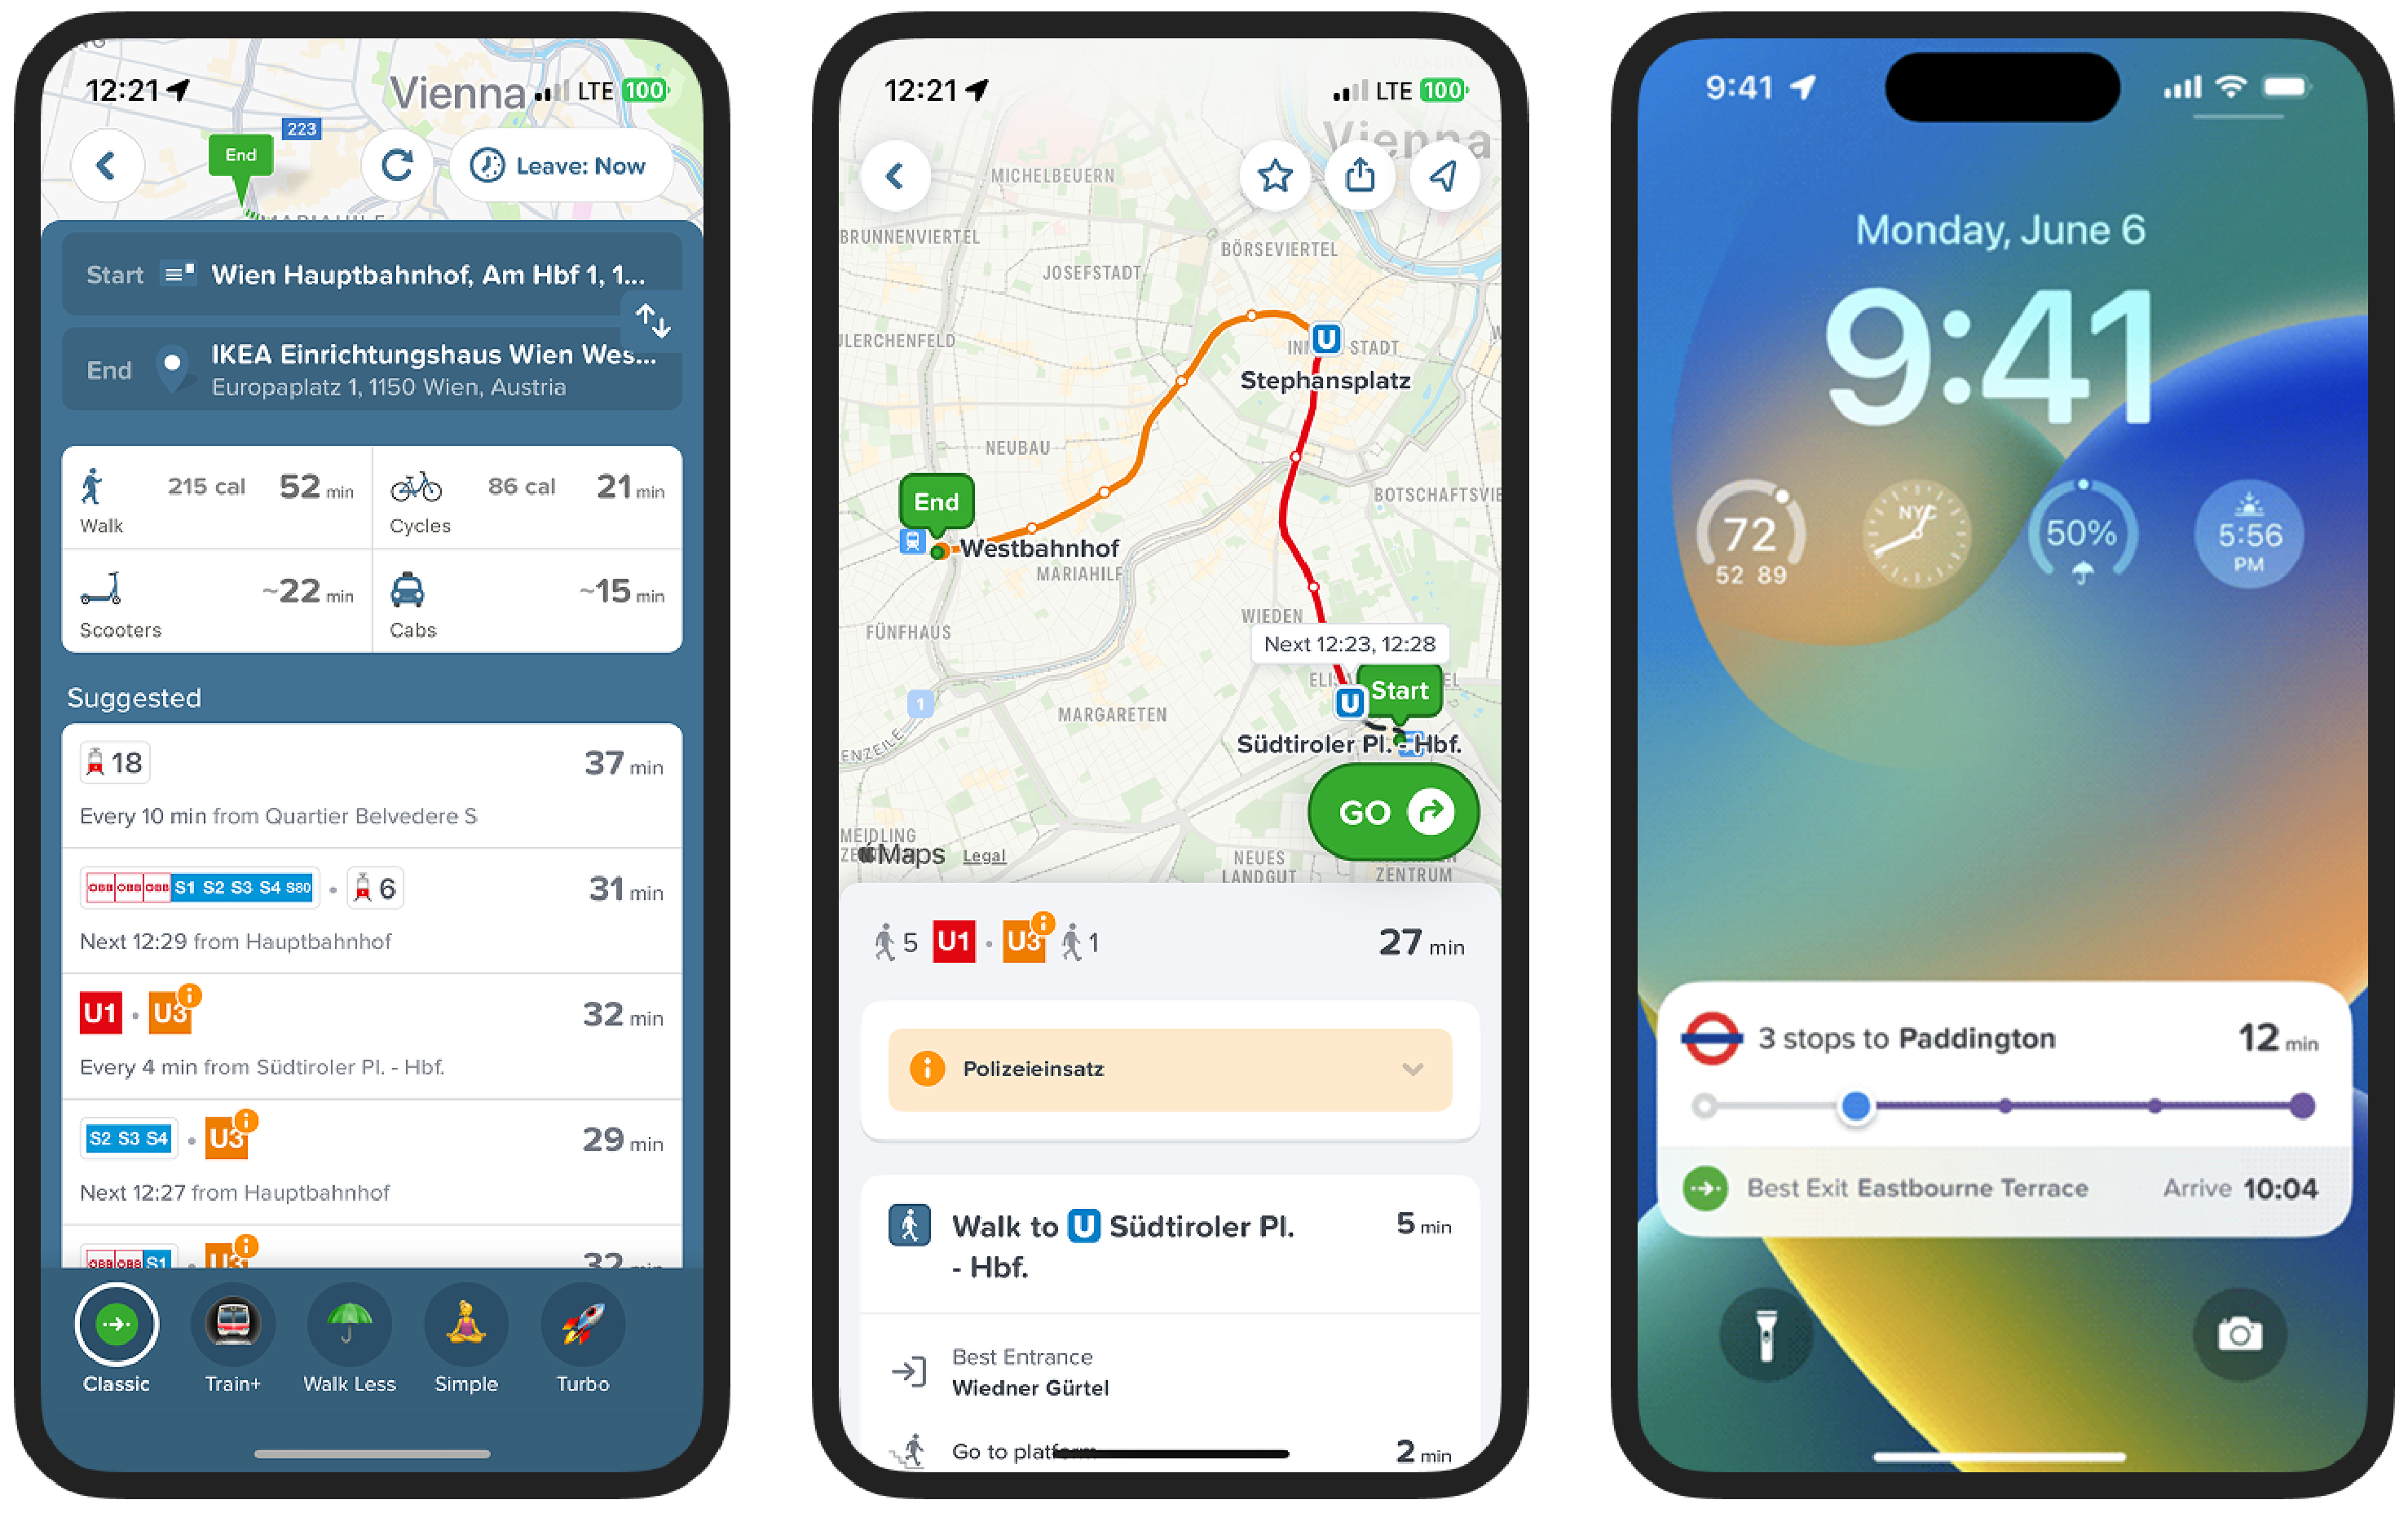
\includegraphics[width=0.7\textwidth]{Citymapper.pdf}
    \caption{Citymapper's Live Activities (left) and Get Off Alerts (right) on iOS}
    \label{fig:Citymapper}
\end{figure}

\section{Moovit}
Moovit is a public transportation navigation app launched in 2012 for iOS, Android and web browsers.
It aims to help users navigate cities by integrating multiple forms of transport including public transit, shared bikes, ride-hailing services and scooters into a single application.
As of 2025, Moovit serves over 1.7 billion users in 3,500 cities across 112 countries and supports 45 languages, according to their website \cite{moovit_about}.

When a user selects a public transit route, Moovit provides Live Activities and notifications to alert them when to get off a bus or train.
Three notifications are sent at different points along the journey, with increasingly urgent messages to ensure the user is informed in time.
During testing, Moovit maintained a stable location signal on the same routes where Citymapper lost connection and effectively communicated the approaching destination both through Live Activities and notifications, as shown in Figure \ref{fig:Moovit}.
However, Moovit also does not provide an audible alarm.

\begin{figure}[htbp]
    \centering
    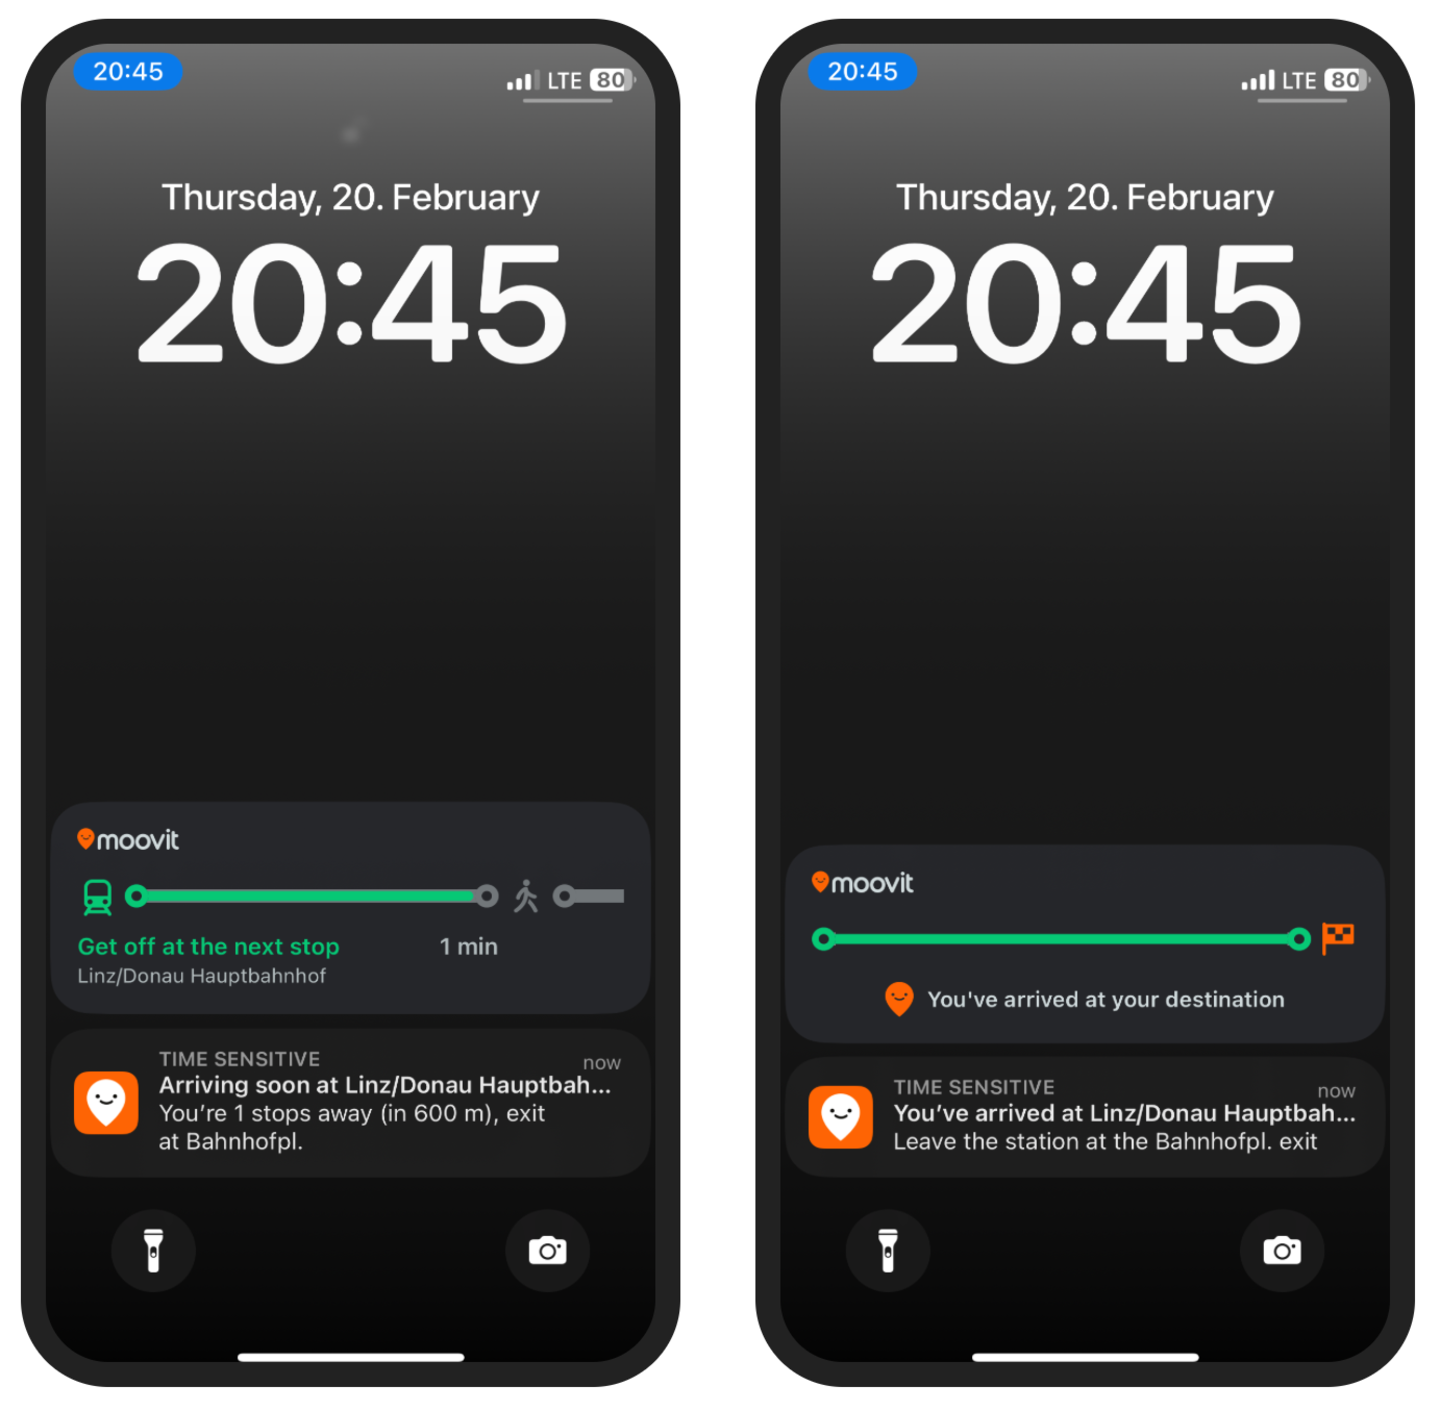
\includegraphics[width=0.7\textwidth]{Moovit.pdf}
    \caption{Moovit's Live Activities and stop notifications on iOS}
    \label{fig:Moovit}
\end{figure}

\section{Conclusion}
The reviewed apps all provide route planning and tracking but differ in how they notify users when to exit public transportation.
Google Maps offers Live Activities on iPhones for navigation updates on the lock screen, though this feature is not globally available.
While stop notifications were reportedly available in 2017, they can no longer be found in the 2025 version of the app.
Citymapper includes stop notifications and Live Activities but frequently lost location tracking, resulting in missed alerts.
Moovit reliably provides stop notifications and Live Activities, making it the most effective at alerting users of their approaching destination.
However, none of these apps offer vibrations or alarms in addition to stop notifications, as proposed in this thesis.